\documentclass[25pt, a0paper, portrait, blockverticalspace=1.5cm]{tikzposter}
\usetikzlibrary{positioning}

\title{\parbox{\linewidth}{\centering Spin Motion Perturbation Effect on the EDM Statistic in the Frequency Domain Method}}
\author{A.E. Aksentyev\textsuperscript{1,2,3}, Y.V. Senichev\textsuperscript{3}}
\institute{
  \textsuperscript{1} National Research Nuclear University ``MEPhI,'' Moscow, Russia \\
  \textsuperscript{2} Institut f\"ur Kernphysik, Forschungszentrum J\"ulich, J\"ulich, Germany\\
  \textsuperscript{3} Institute for Nuclear Research of the Russian Academy of Sciences, Moscow, Russia
}


\usetheme{Simple}
\usecolorstyle{Russia}
\colorlet{blocktitlefgcolor}{black}

\usepackage{mathtools}
\usepackage{amsmath}
\usepackage{xparse}
\usepackage{caption}
\captionsetup{font=large}
\usepackage{multicol}
\setlength\columnsep{1.5cm}


\let\oldvec\vec
\renewcommand{\vec}{\boldsymbol}
\DeclareDocumentCommand{\bkt}{sm}{\IfBooleanTF{#1}{\left[ #2 \right]}{\left(#2\right)}}
\DeclareDocumentCommand{\ddt}{m}{\frac{\mathrm{d} {#1}}{\mathrm{d} t}}
\DeclareDocumentCommand{\pddx}{mO{t}O{}}{\frac{\partial^{#3} {#1}}{\partial {#2}^{#3}}}
\newcommand{\w}{\omega}
\newcommand{\W}{\Omega}
\newcommand{\avg}[1]{\langle {#1} \rangle}
\newcommand{\nbar}{\bar n}
\newcommand{\ntrn}{n_{turn}}
\newcommand{\const}{\mathrm{const}}

\begin{document}

\maketitle

\block{INTRODUCTION}{
  \begin{multicols}{3}
    The Frequency Domain method of search for the EDM of a particle consists in measuring the combined
    MDM+EDM spin precession frequency in two situations: beam circulating clockwise (direct), and
    counter-clockwise (time-reversed). When these frequencies are added up, the MDM effect cancels, leaving
    only the EDM in the final statistic.\columnbreak

    The frequency in question is estimated by fitting a sine function to polarimetry data. However, variation of
    the spin precession angular velocity vector introduces a mismatch between the constant-parameter sinusioidal
    model and measurement data.\columnbreak

    Model specification errors are prone to introducing biases into parameter estimates.
    The purpose of this work is to analyze the effect of spin motion perturbation on the EDM statistic.
  \end{multicols}

}

\begin{columns}
  \column{.5}
  \block[bodyoffsety=2cm, titleoffsety=2cm]{PROBLEM STATEMENT}{
    Solution of the T-BMT equation for the
    vertical spin-vector component:
    \begin{equation}\label{eq:master}
      s_y(n_{turn}) = \sqrt{\bkt{\nbar_y\nbar_z}^2 + \nbar_x^2}\cdot\sin\bkt{2\pi\nu_s\cdot\ntrn + \delta}.
    \end{equation}
    Here
    \begin{itemize}
    \item the \emph{invariant spin axis} $\nbar$ defines the orientation of the spin precession angular
      velocity vector;
    \item \emph{spin tune} $\nu_s$ defines the magnitude of the vector.\\
    \end{itemize}

    Data is fitted by model
    \[
    f(t) = a\cdot\sin(\w\cdot t + \delta),
    \]
    $(a,\w,\delta)=\const$.\\

    Therefore, significant variation of $\nbar$ and/or $\nu_s$ can lead to model specification error.
  }

  \block[bodyoffsety=1.5cm, titleoffsety=1.5cm]{SIMULATION}{
    \begin{tikzfigure}
      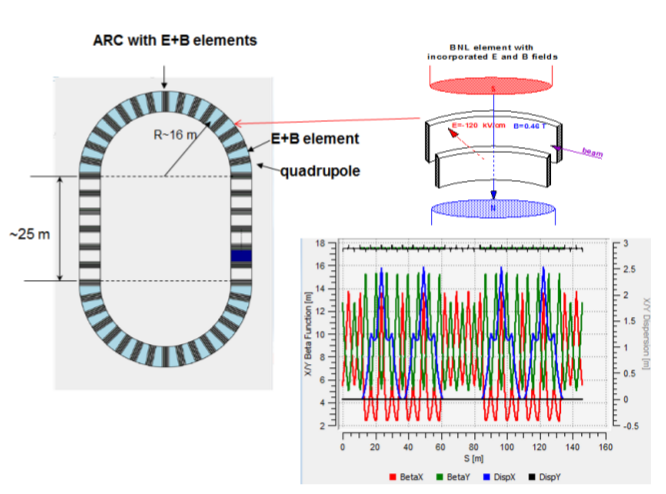
\includegraphics[width=\linewidth, trim=0 0 0 50, clip]{../img/Lattice/BNL}
    \end{tikzfigure}
    \captionof{figure}{Imperfect Frozen Spin lattice in which sextupole spin decoherence suppression is
      implemented}
    \vspace*{1cm}

    \begin{minipage}[t]{.5\linewidth}
      \textbf{Machine imperfections}
      \begin{itemize}
      \item rotations of E+B spin rotator elements about the optic axis by
        $\alpha \sim N(\mu_i, 3\cdot 10^{-4})$ degrees;
      \item $\mu_i \in [-1.5\cdot10^{-4}, +2.5\cdot10^{-4}]$ degrees;
      \item $\mu_i$ simulates the application of a Spin Wheel.
      \end{itemize}
    \end{minipage}~~~~~~
    \begin{minipage}[t]{.5\linewidth}
      \textbf{Particle}
      \begin{itemize}
      \item 0.3 mm offset from the reference orbit --- vertical plane betatron oscillations;
      \item injection kinetic energy slightly off Frozen Spin;
      \item small $\nbar_x$ value --- increased sensitivity to perturbations.
      \end{itemize}
    \end{minipage}
  }
  \block{CONCLUSIONS}{
    \textbf{Three circumstances} of the betatron motion effect on the EDM statistic:
    \begin{enumerate}
    \item $\nbar$ variation is insignificant compared to $\nu_s$ variation.
    \item $\sigma[\epsilon_2] \ll \sigma[P_y]$.
      Therefore, the superposition of this systematic error with random measurement error will
      exhibit no statistically-significant systematicity.
    \item $\sigma[\hat a, \hat\w] < 10\%$.
      Even if $\nbar$ variation happens to be sufficiently strong to affect $\hat a$-estimate, 
      its effect on $\hat\w$ will be reduced by at least a factor of 10.
    \item This systematic effect is controllable.
      The advantage of Frequency Domain versus Space Domain is that by increasing the SW roll rate
      the $\nbar$ oscillations can be continuously minimized.
    \end{enumerate}
  }

  \column{.5}
  \block[bodyoffsety=2cm, titleoffsety=2cm]{ANALYSIS}{
    \begin{minipage}[t]{.6\linewidth}
      \textbf{Three data series}
      \begin{itemize}
      \item[TRK] spin data generated by the COSY INFINITY TR command (closest to measurement data);
      \item[GEN] data computed from equation~\eqref{eq:master} with $\nbar$, $\nu_s$ the
        TSS command output (accounts for parameter variation remaining within the confines of
        the sinusoidal model);
      \item[IDL] as in GEN, but $\nbar = \avg{\nbar(t)}$, $\nu_s = \avg{\nu_s(t)}$ (closest to the model).
      \end{itemize}
    \end{minipage}~~~~~~~~~~~~~~
    \begin{minipage}[t]{.3\linewidth}
      \textbf{Two comparator statistics}
      \begin{itemize}
      \item $\epsilon_1(t) = s_y^{gen}(t) - s_y^{idl}(t)$;
      \item $\epsilon_2(t) = s_y^{trk}(t) - s_y^{idl}(t)$.
      \end{itemize}
    \end{minipage}
    \vspace*{1cm}\\
    \begin{minipage}[t]{\linewidth}
      \textbf{What was done}
      \begin{itemize}
      \item Compared model~\eqref{eq:master}'s goodness-of-fit with respect to $S_y^{trk}$, $S_y^{gen}$, $S_y^{idl}$;
      \item checked $\epsilon_1$ and $\epsilon_2$'s standard deviation behavior against $\sigma[\nbar]$ behavior.
      \end{itemize}
    \end{minipage}
  }
  \block{RESULTS}{
    \begin{tikzfigure}
      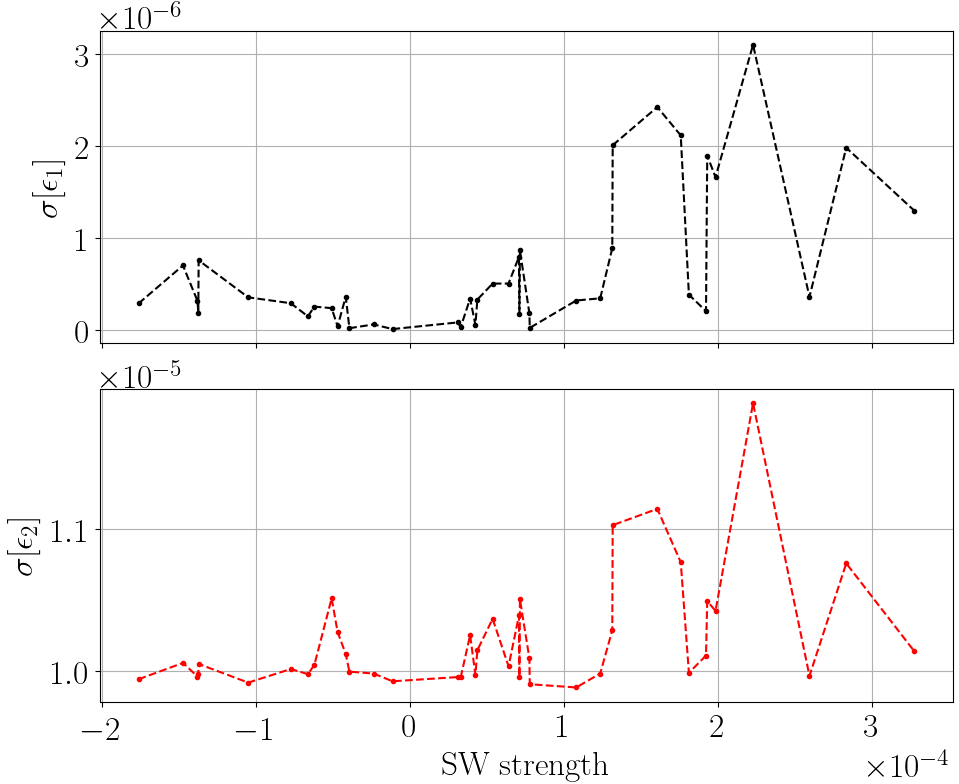
\includegraphics[width=.9\linewidth]{../img/IPAC19/residual_SD_vs_SW(both)}
    \end{tikzfigure}
    \captionof{figure}{Residual standard deviations versus Spin Wheel roll rate}
    \begin{tikzfigure}
      \includegraphics[width=.9\linewidth]{../img/IPAC19/NBAR_variation_SD_vs_SW}
    \end{tikzfigure}
    \captionof{figure}{$\nbar$ components' standard deviations versus Spin Wheel roll rate}
  }

  %% \block{REFERENCES}{
  %%   \begin{thebibliography}{9}
  %%   \bibitem{Senichev:2017amn} 
  %%     Y.~Senichev, A.~Aksentev, A.~Ivanov and E.~Valetov,
  %%     %``Frequency domain method of the search for the deuteron electric dipole moment in a storage ring
  %%     %with imperfections,''
  %%     arXiv:1711.06512 [physics.acc-ph].
  %%     %%CITATION = ARXIV:1711.06512;%%
  %%   \end{thebibliography}
  %% }
\end{columns}


\end{document}
